% !Mode:: "TeX:UTF-8"

\chapter{基于消息传递的人对间关系网络}
\label{ch:model}

本章将提出一个消息传递的人对间关系网络,简称PPRN。本章节将说明PPRN网络的特征提取模块、消息传递模块和消息池化模块,以及结合周边物体信息的模块,最后定义整个模型的优化方法和具体实现细节。


\section{基本框架}
首先,需要提到的是PPRN的输入和现有的模型是存在一些差别。对于Dual-glance和GRM模型来说,输入是一张图片,两个人的包围盒坐标。在第一章的介绍中提到,本文的出发点是希望对人对间的关系进行建模。对于图像的社会关系理解任务,需要识别出图片上每个人对之间的社会关系,但是图像特征的模糊性和不确定性,这是一个很难的任务。利用上图上人对之间的关系信息,即结构信息或场景信息。在经过特征提取模块得到的关系编码已经包含了浅层的类别类别状态,而对图片上每个人对间关系交互进行建模,是在识别的基础上的高层次的推理。因此,PPRN网络的输入是以图片为单位而不是人对,每次同时输出一张图片上所有人对间的社会关系。PPRN主要是由4个模块组成,并且模型的主要预算模块是向量,以下提到的所有向量编码维度均为n维。如果将人之间的社会关系视作节点,本文对于图片上所有这样关系节点的全连接图成为{\it 社会关系图谱},节点间的连边不含语义,采用类似于GRM的方式,利用特征提取模块得到的编码来初始化社会关系图谱上的关系节点。人对关系采用GRU来探索一个节点和图上其它节点间的交互,一张图片往往是一个场景,使用场景中其它节点的社会关系来对当前节点的社会关系消歧。此外,引入池化机制探索不同节点交互时的影响力。

首先,本文的模型包括两个版本,分别是PPRN-(obj region),简称为PPRN,如图\ref{fig:model-pprn}所示,PPRN模型是一个端到端的架构,特别需要说明的是PPRN不包括周边物体信息模块。PPRN模型接受一张图片和图片上所有人的包围盒的作为输入,经过前文提到的3 个模块,并且每个模块的作用各有分工。模型首先提取图片中关于人和人对包围盒的特征,图\ref{fig:model-pprn} 中的$p_{uij}$表示图上第i-th 个人和第j-th 个人的联合区域。$b_{i}$表示第i-th个人的包围和的坐标和包围盒的面积编码。在消息池化模块中,消息池化函数计算关系间的消息,然后作为下一轮GRU 神经元的输入。其中$\oplus$ 表示一个可学习的权重参数。而对于消息传递模块,通过循环神经网络来实现通过反复传递消息来提醒当前节点目前场景中其它节点的行为,这个是图推理的一种实现方式,可以优化对社会关系的估计。在最后一次迭代时,利用GRU神经元最后的隐藏层的输出连接一个全连接层得到最后的包含场景特征的编码$F_{rel}$。
\begin{figure}[htpb]
	\centering
	%	\includegraphics[width=0.48 \textwidth, trim=10 10 10 80,clip]{./pic/example_new.pdf}
	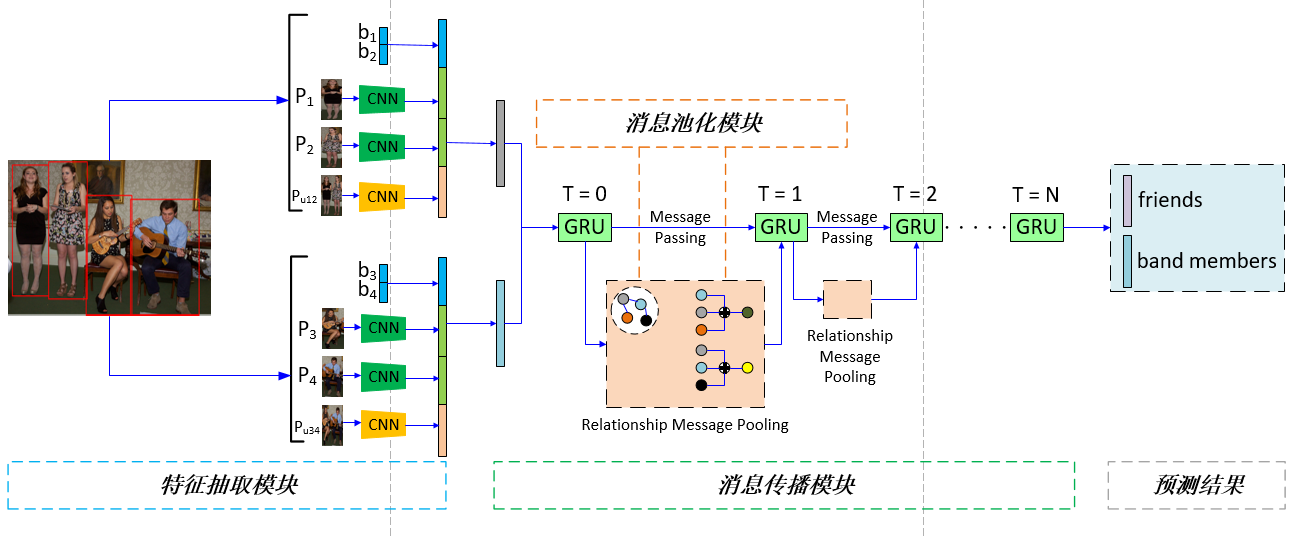
\includegraphics[width=0.98 \textwidth,clip]{model.png}
	%\hspace{0.02\textwidth}
	%\vspace*{-0.08cm}
    \caption{PPRN模型的结构示意图}
	\vspace*{-3.5mm}
	\label{fig:model-pprn}
\end{figure}

\subsection{特征抽取模块}


模型微调是指给定一个预训练模型,这里的预训练网络通常是在大规模标注数据集上训练好的模型,例如常用的预训练模型有Vgg和ResNet。 此时的模型已经能很好的抽取大部分图片的信息,比如卷积神经网络的浅层往往是提取基础特征,例如边缘、轮廓等基础特征。深层卷积层提取抽象特征,例如脸型,而最后的全连接层根据特征组合进行连接分类。对于在大规模数据集上已经训练过的模型来说,已经具备了提取浅层特征和深层次抽象特征的能力。基于预训练的模型来新的数据集能节省很多的计算时间和计算资源,而且还能提升模型的效果。常见的模型微调方法是将我们现有的分类层替代预训练模型的最后一层,然后以较小的学习率微调前面的所有层,原因是不想过快的扭曲前面已经学习好的特征,然后着重训练最后的分类层。或者冻住预训练模型前面的若干层,微调后面的网络层。

特征提取模块包括物体的特征和人对的特征,对于人对的特征,采用的预训练模型是ResNet-101\cite{he2016deep},本文的做法微调ResNet-101模型的后2层和最后分类层。特征抽取模块的主要目标是提取出输入的图片和人的包围盒坐标区域的图像特征。因此,该模块首先修剪出三个小块,$p_1$ 和$p_2$ 为个体的区域,$p_{u}$ 为两个人区域的并集区域,这些区域的特征包含了用于识别关系的基本组成部分。这些区域首先被调整为大小224 $\times$ 224,然后输入三个ResNet,其中$p_1$ 和$p_2$ 的区域的网络是共享参数的。三个模型最后一个卷积层的输出拼接在一起,形成视觉特征向量$\mathbf{v}_1$。 其次,位置信息同样很重要,对于其中的关系类别中的`` 无关系'',这单纯从视觉特征来判断是很难的,此时位置信息往往能起到很好的区分作用。我们表示一个包围盒$i$ 的特征为$b_i^{pos}$ = $\{ x_{i}^{min}, y_{i}^{min}, x_{i}^{max}, ~y_{i}^{max},~ area_{i} \}$ $\in$ $R^5$。 其中这些值都是相对位置。$x_{i}^{min}$和$y_{i}^{min}$是包围盒的左上角坐标,$x_{i}^{max}$和$y_{i}^{max}$是右下角坐标。最后这些特征拼接在一起后通过全连接层形成关系特征向量$\mathbf{v}_h$


\subsection{消息传递模块}

对于一张图片中$n$个人对的关系,通过特征抽取模块,得到了图片中所有人对关系的特征编码,$\{ \mathbf{v}_{1},\mathbf{v}_{2},...,\mathbf{v}_{n} \}$,并且对于一张图片构成的社会关系图谱,是一张全连接图。对于特征抽取模块得到的关系向量编码通过如公式\ref{eq:model-hidden-init}所示,转换到一个低维空间,其中$ \varphi_{rel} $ 可是视为全连接层。
\begin{equation} \label{eq:model-hidden-init}
    h_{i}^{0} = \varphi_{rel} (v_{i})
\end{equation}

为了学习到图片中的场景信息信息对关系编码的约束,我们采用了循环神经网络来执行社会关系检测理解的推理工作。与Zheng\cite{zheng2015conditional}的模型不同的是,我们采用通用的RNN 神经元来计算隐藏层状态。相比较LSTM,GRU少了一个门,因此更加简单并且参数较少,学习起来更快,因此本文采用的是GRU模块。我们采用第t步的隐藏层状态编码表示社会关系图谱中所有关系节点信息,关系节点的向量编码会随着RNN 序列的长度每一步都更新。而关键的是每一步GRU的输入来自消息池化模块的输出,消息池化模块承担着关系节点间交互的任务。具体细节如公式\ref{eq:model-gru}所示,其中$\mathbf{v}_h$会当作GRU 第一步的输入,并且此时的隐藏层的初始化为值为0的向量。这里的$\sigma$和$tanh$分别表示逻辑斯谛回归和双曲正切函数。$\odot$操作表示点乘操作,$\bm{r}_t$表示重置门,$\bm{z}_t$表示更新门,下标$t$表示迭代步骤。$\mathbf{W}_r$和$\mathbf{W}_z$ 表示两个门需要的参数,这些参数可训练的。

\begin{equation} \label{eq:model-gru}
\begin{split}
\bm{r}_t &=  \sigma(\bm{W}_{r}[\bm{h}_{t-1}, \bm{x}_t]), \\
\bm{z}_t &=  \sigma(\bm{W}_{z}[\bm{h}_{t-1}, \bm{x}_t]), \\
\hat{\bm{h}_t} &= tanh(\bm{W}[\bm{r}_t \odot \bm{h}_{t-1}, \bm{x}_{t}])\\
\bm{h}_t &= (1 - \bm{z}_t) \odot \bm{h}_{t - 1} + \bm{z}_t \odot \hat{\bm{h}_t} \\
\end{split}
\end{equation}

\subsection{消息池化模块}

消息传递模块利用RNNs解决推理问题,但是在每个迭代步的时候,GRU单元会接受多个来自社会关系图上其他节点的消息,需要有一个聚合模块来将这些信息结合成一个有意义的编码向量。直观来看,常见的池化能实现这个功能,例如常用的最大池化和平均池化。在理解当前图片的社会关系图谱时,只利用上下文的结构信息中最相关的那部分是最合理的方式。而本文的消息池化模块也是出于这个目的提出的。下面将会说明简要说明注意力机制的基本情况。如公式\ref{eq:model-mp-atten}所示,其中第$t$ 步的节点$i$的前一步隐藏层状态为$h_{i,t-1}$,$m_{i,t}$表示来自其他节点消息的聚合,而$\bm{m}_{i,t}$ 将会作为第$t$ 步中公式
\ref{eq:model-gru}中输入,即$\mathbf{x}_{t}$。其中符号[.]表示两个向量编码的拼接,$\sigma$表示激活函数,$\bm{w}$是需要学习的参数向量,$\bm{h}_{j \to i,t-1}$是节点j在第t-1步时的隐藏层编码,并且等同于
公式\ref{eq:model-gru}中节点j的$h_{t-1}$

\begin{equation}
    \label{eq:model-mp-atten}
	\bm{m}_{i,t} = ~\sum_{j\neq i} \sigma{(~\bm{w}^T[~\bm{h}_{i,t-1},\bm{h}_{j \to i,t-1}~]) \bm{h}_{j \to i,t-1}}	
\end{equation}

%%%%%%%  注意力机制  %%%%%%%%%%%%


\subsection{结合周边物体信息模块}

%%%%%%%%%%%%%% 之后写  %%%%%%%%%%% 先空着
本文在模型PPRN,如图\ref{fig:model-pprn}的基础上,本文实现了类似Dual-glance的方法结合周边物体信息模块,模型简称为PPRN+(obj region),如图\ref{fig:model-atten}。当前模块主要包括两个步骤,利用faster-rcnn 中的RPN(region proposal network) 网络模块生成物体置信度高的区域,其次利用注意力机制得到关于周边物体区域的特征。

在一张图片中,往往会存在一些日常见到的物体,例如桌子、电脑、杯子,如果在一张图片中检测到了被杯子、床或者桌子等物体,那么当前的社会关系往往是``家庭''。因此本文在利用关系上下文的基础上,进一步加入周边物体信息来提升效果。但是在PISC 和PIPA-relation数据集中,不包含物体包围盒的标注以及物体类别的标注。但是COCO\cite{lin2014microsoft}是一个大规模的物体检测的数据集,覆盖了日常常见的80类物体。采用在COCO上预训练好的faster-rcnn 模型,利用其中的区域生成网络。区域生成网络的输入可以是任何大小的图片,输出是一些长方形的检测框,其中每个检测框都带有是否包含物体的得分。由于期望RPN和fast-rcnn 共享有vgg\cite{simonyan2015very} (本文采用vgg,也可采用其他的预训练模型)生成的特征图,这里的vgg 网络有13个可训练的卷积层。
\begin{figure}[htpb]
	\centering
	%	\includegraphics[width=0.48 \textwidth, trim=10 10 10 80,clip]{./pic/example_new.pdf}
	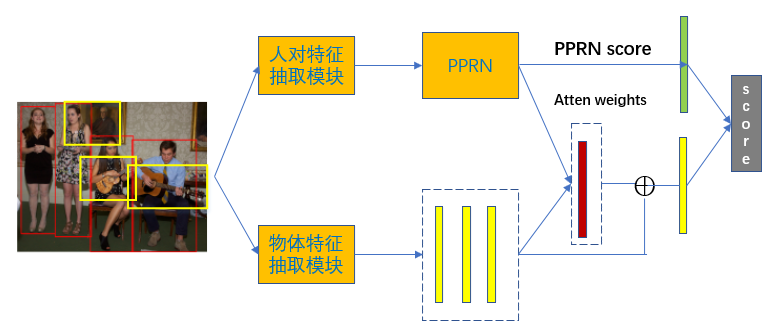
\includegraphics[width=0.98 \textwidth,clip]{model-atten.png}
	%\hspace{0.02\textwidth}
	%\vspace*{-0.08cm}
    \caption{PPRN模型的结构示意图}
	\vspace*{-3.5mm}
	\label{fig:model-atten}
\end{figure}

经典的方法生成检测框都非常耗费时间,例如RCNN和fast-rcnn采用的选择性搜索,而faster-rcnn 抛弃传统的方法,直接从特征图生成检测框,能极大的提升检测的速度。如图\ref{fig:rpn},可以看到RPN网络由两个模块组成,上面的模块为物体的前后景分类,检测的目标为前景。下面的模块为检测框区域坐标的回归,用于获得更精准的检测框,proposal层结合检测框的坐标和前景类别获取在图上的区域,这两个模块结合起来相当于完成了目标定位的功能。具体执行步骤如下:
\begin{enumerate}
    \item 对于,vgg 特征提取模块得到$d$张特征图,相当于每个点都是d-dimensions。
    \item 对于$d$张特征图,首先经过$3 \times 3$的卷积核的处理,用于结合周边的空间信息,同时每个点对应的d-dimension不变。
    \item 假设在$d$张特征图中每个点上有k个锚点,每个锚点分为前景和后景,所以在前后景分类中,d-dimension的特征向量转化为一个2k的得分向量,而每个锚点都有四个坐标的偏移量,对于检测框回归模块,特征向量转化为4k的得分向量。其实RPN就是在和原图相同的尺寸上,设置密密麻麻的候选锚点。然后用cnn网络来判断哪些是包含物体目标的前景,那些是不包含物体目标的后景。
    \item 全部锚点框都拿去训练太多了,因此会在锚点框中随机选取128个positive的锚点框和128个negative锚点框用于训练
\end{enumerate}
\begin{figure}[htpb]
	\centering
	%	\includegraphics[width=0.48 \textwidth, trim=10 10 10 80,clip]{./pic/example_new.pdf}
	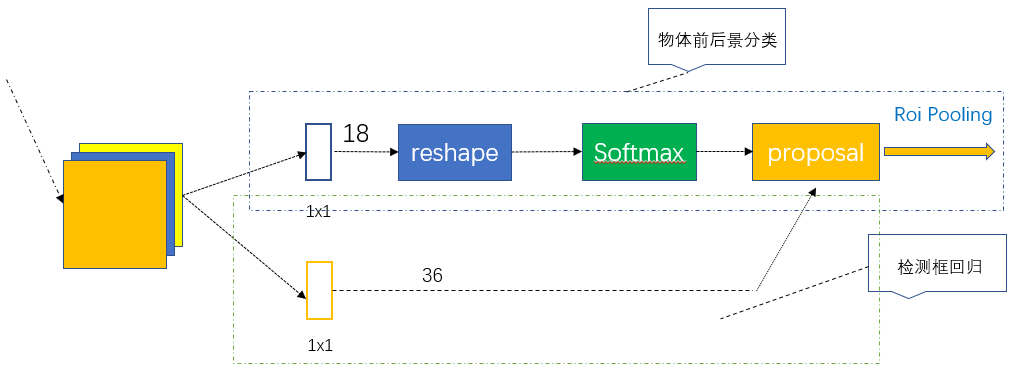
\includegraphics[width=0.95 \textwidth,clip]{rpn.png}
	%\hspace{0.02\textwidth}
	%\vspace*{-0.08cm}
    \caption{RPN网络结构示意图}
	\vspace*{-3.5mm}
	\label{fig:rpn}
\end{figure}
上文提到的锚点框,其示意图如图\ref{fig:anchor}其实就是对于特征图的每个点生成一组检测框,检测框的尺寸由输入的图片的尺寸决定的,在本文中,对于每个检测点生成3种尺寸,每种尺寸3种形状的锚点框。这也是常见的多尺度方法,这9个初始的锚点框的准确度由RPN的区域回归模块处理。对于生成的检测框,因为尺度是原图的尺度大小,需要映射为特征图的尺度大小,Roi pooling层划分出非均匀的网格,对网格采用最大池化然后得到锚点框的特征向量。
\begin{figure}[htpb]
	\centering
	%	\includegraphics[width=0.48 \textwidth, trim=10 10 10 80,clip]{./pic/example_new.pdf}
	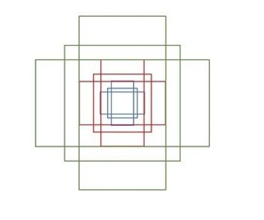
\includegraphics[width=0.50 \textwidth,clip]{anchor.png}
	%\hspace{0.02\textwidth}
	%\vspace*{-0.08cm}
    \caption{anchor示意图}
	\vspace*{-3.5mm}
	\label{fig:anchor}
\end{figure}

利用前文提到的RPN网络,对于图片$\bm{I}$,生成是前景的检测框,并且过滤掉IOU(Intersection-over-Union)低于超参数$\tau_{u}$的检测框,得到一组检测框$\bm{P}_{I}$,采用预训练的vgg来得到特征图$conv(I)$,对这里的每个检测框,经过一层Roi pooling 层得到固定长度的物体区域特征$\mathbf{v}$,对于图片所有的检测框,从$conv(I)$生成$\{ \mathbf{v}_{i}|i=1,2,....,N\}$特征向量,对于关系来说,和它关联的物体是比重是不同的,例如对于关系``家庭'',``碗''的权重比``桌子''的权重大的多,所以我们期望对于不同的物体区域引入不同的权重系数。因此,在当前模块中,引入注意力机制
(attention mechanism),经过消息传递和池化的关系的特征编码$\mathbf{v}_{top}$和物体特征编码$\mathbf{v}_{i}$共同决定权重系数的值:
\begin{equation}
    \mu_{i} = \mathbf{u}^{T}~tanh(~\mathbf{W}_{r}v_{top}+\mathbf{W}_{o}v_{i}~)
\end{equation}
\begin{equation}
    \mathbf{a}_{i} = softmax(\mu_i) = \frac{exp(\mu_{i})}{\sum_{j}^{N}exp(\mu_{j})}
\end{equation}
根据关系得到每个物体区域特征的权重后,各个区域权重分别与物体区域的特征编码相乘,如公式\ref{eq:model-obj-wei}所示:
\begin{equation}
    \label{eq:model-obj-wei}
    \mathbf{v}_{att} = \sum_{i}\mu_{i}~\mathbf{v}_i
\end{equation}
最终用于分类的的编码由是将消息传递、池化模块得到的关系编码向量$v_{top}$,和带权物体特征编码特征向量$\mathbf{v}_{att}$,最终的分类层函数如公式\ref{eq:model-cls}:
\begin{equation}
    \label{eq:model-cls}
    \mathbf{s} = \mathbf{W}_{c}[~\mathbf{v}_{top}~,~v_{att}~] + \mathbf{b}
\end{equation}

\subsection{优化和实现细节}

对于图片\textbf{I}的第k个人对,模型预测出的的得分为$\mathbf{s}_{I,k} \in \mathcal{R}^{|\mathcal{C}|}$,我们采用{\it softmax}函数对得分进行归一化来得到每个类别的概率$\mathbf{p}^{I,k} \in \mathcal{R}^{|\mathcal{C}|}$,如公式\ref{eq:model-prob-eq}所示:
\begin{equation}
  \label{eq:model-prob-eq}
  p_i^{I,k} = \frac{\exp{s_i^{I,k}}}{\sum_{j=1}^{|\mathcal{C}|}{\exp{s_j^{I,k}}}}, i=1,2,\dots,|\mathcal{C}|
\end{equation}
这里的$\mathcal{C}$表示社会关系的类别,$|\mathcal{C}|$表示类别的数量,由于是分类任务,模型最终的损失函数如公式\ref{eq:model-loss-eq},其中$N(I)$表示图片I的人对数量,L(.)表示交叉熵损失函数,$\mathcal{I}$ 表示整个图片集合。
\begin{equation}
  \label{eq:model-loss-eq}
  \mathcal{L} = - \frac{1}{\sum_{I \in \mathcal{I}}\text{N}(I)} \sum_{I \in \mathcal{I}} \sum_{k=1}^{\text{N}(I)} \sum_{i=1}^{|\mathcal{C}|} \text{L}(y_{i}^{I,k}, p_{i}^{I,k})
\end{equation}

关于本文中提到的预训练模型ResNet-101和vgg-16,使用的均是由深度学习框架pytorch提供的。并且在数据集PISC-fine和PIPA-relation中存在类别不均衡问题,PISC-fine类别分布如表
\ref{tab:model-pisc-cls},在实际训练过程中,我们采用常见的过采样和降采样的方法来构造最终的训练集,例如对于PISC-fine中类别为``Commercial''的关系,我们增加3倍的样本,并且这些样本的人对会互换位置(例如p1和p2 是Commercial,那么新增加的样本为p2和p1也是Commercial)。

在本文中,最开始微调RestNet-101提取人对信息时候采用的是优化方法是SGD(Stochastic Gradient Descent),不同数据集在微调所需要的迭代次数是不一样的,同时由于本文模型的输入是以图片为单位,但是不同图片的人对数量是不一样的,所以batch\_size也是不一样的。首先,微调不同数据集所需要迭代次数如表\ref{tab:model-ft-epoch},上文同样提到了,综合考虑到效率和模型效果,本文采用的方法是微调网络最后两个卷积层,其他层的参数冻结,不参与学习更新。其次,利用前面微调的模型参数,固定住,然后只更新消息传递和池化模块的参数,这个步骤采用的优化算法是Adam\cite{kingma2014adam},不断迭代直到模型收敛。\textbf{PPRN}模型用pytorch实现,训练时每个mini-batch会包含24张图片,每个epoch需要的时间是200ms。

\begin{table}[htpb]
  \centering
  \caption{PISC-fine类别分布表}
  \label{tab:model-pisc-cls}
  \begin{tabular}{c|c|c|c|c|c|c}
    \toprule
    关系类别 & Friends & Family & Couple & Professional & Commercial & No Relation \\
    \midrule
    样本数量 & 12686 & 788 & 1552 & 20842 & 523 & 11979 \\
    \bottomrule
  \end{tabular}
\end{table}

\footnote{https://download.pytorch.org/models/vgg16-397923af.pth}
\footnote{https://download.pytorch.org/models/resnet101-5d3b4d8f.pth}
\footnote{https://pytorch.org/}

\begin{table}[htpb]
  \centering
  \caption{fine-tune ResNet-101需要的迭代轮数}
  \label{tab:model-ft-epoch}
  \begin{tabular}{c|c|c|c}
    \toprule
    数据集 & PISC-coarse & PISC-fine  & PIPA-relation \\
    \midrule
    迭代轮数 & 17 & 24 & 2 \\
    \bottomrule
  \end{tabular}
\end{table}

\section{本章小结}

本章提出了一个全新的基于消息传递机制的关系网络,简称\textbf{PPRN}。\textbf{PPRN}模型是一个端到端的架构,主要由四个部分构成,特征抽取模块、消息传递模块、消息池化模块、结合物体信息模块,模块之间是串联的,并且它们的作用和分工不同。

特征抽取模块的作用是输入一张图片,图片中所有人身体的检测框坐标,提取出其中表示人对关系的基本特征编码,包括单个人区域、两个人的联合区域和位置信息,特点是利用两个不同的预训练模型来处理单人区域和两个人的联合区域,我们同时结合了图像特征和位置特征,特征提取采用的是微调后的ResNet-101。基于特征提取模块得到的向量编码已经能够表达人对间的社会关系了,而消息传递和池化模块的作用是结合当前图片的场景信息进行关系类别推理,学习到图片中不同人对关系之间约束。学习这个约束的原因是,在一张图片中,场景往往是固定的,所以图片中不同人对的社会关系之间是相互影响的。本文采用以GRU为基础的RNN 作为推理模型,每次迭代时,利用注意力机制结合图片中其它人对关系的编码,实现不同人对关系间的消息传递,RNN最后一步的隐藏层编码表示所有的人对关系。

然后,本章在Dual-glance模型的基础上,实现了类似的结合物体信息模块。物体信息指的是利用基于大规模训练集的预训练faster-rcnn模型,RPN网络生成图片的物体检测框,包含物体的概率大于一定的阀值。本章详细的介绍了RPN网络的细节,如何生这些检测框坐标。最后提取出这部分上下文物体区域的信息。因为不同物体区域对和不同的社会关系的相关度不一样,同样利用注意力机制为每个物体区域的特征编码分配权重。

最后,本章介绍了优化和实现细节。优化主要是采用常见的交叉熵损失函数,并且针对PISC-fine和PIPA-relation数据集的数据不均衡问题,进行数据上的过采样和降采样。模型的训练过程是分段式的,包括微调预训练模型和本文提出的模块训练两部分,结合不同的学习率和优化方法模型得以训练。




